\documentclass{beamer}
\usepackage[utf8]{inputenc}

\usetheme{Madrid}
\usecolortheme{default}
\usepackage{amsmath,amssymb,amsfonts,amsthm}
\usepackage{txfonts}
\usepackage{tkz-euclide}
\usepackage{listings}
\usepackage{adjustbox}
\usepackage{array}
\usepackage{tabularx}
\usepackage{gvv}
\usepackage{lmodern}
\usepackage{circuitikz}
\usepackage{tikz}
\usepackage{graphicx}
\usepackage{mathtools}
\setbeamertemplate{page number in head/foot}[totalframenumber]

\usepackage{tcolorbox}
\tcbuselibrary{minted,breakable,xparse,skins}



\definecolor{bg}{gray}{0.95}
\DeclareTCBListing{mintedbox}{O{}m!O{}}{%
  breakable=true,
  listing engine=minted,
  listing only,
  minted language=#2,
  minted style=default,
  minted options={%
    linenos,
    gobble=0,
    breaklines=true,
    breakafter=,,
    fontsize=\small,
    numbersep=8pt,
    #1},
  boxsep=0pt,
  left skip=0pt,
  right skip=0pt,
  left=25pt,
  right=0pt,
  top=3pt,
  bottom=3pt,
  arc=5pt,
  leftrule=0pt,
  rightrule=0pt,
  bottomrule=2pt,
  toprule=2pt,
  colback=bg,
  colframe=orange!70,
  enhanced,
  overlay={%
    \begin{tcbclipinterior}
    \fill[orange!20!white] (frame.south west) rectangle ([xshift=20pt]frame.north west);
    \end{tcbclipinterior}},
  #3,
}
\lstset{
    language=C,
    basicstyle=\ttfamily\small,
    keywordstyle=\color{blue},
    stringstyle=\color{orange},
    commentstyle=\color{green!60!black},
    numbers=left,
    numberstyle=\tiny\color{gray},
    breaklines=true,
    showstringspaces=false,
}

\title 
{4.3.53}
\date{September 15, 2025}


\author 
{Vivek K Kumar - EE25BTECH11062}



\begin{document}


\frame{\titlepage}
\begin{frame}{Question}
The Fahrenheit temperature $F$ and absolute temperature $K$ satisfy a linear equation.
Given that $K = 273$ when $F = 32$ and that $K = 373$ when $F = 212$. Express K in
terms of $F$ and find the value of $F$, when $K = 0$.
\end{frame}

\begin{frame}{Variables used}
\begin{align}
\end{align}
\begin{table}[H]    
  \centering
  \begin{tabular}{|c|c|}
\hline
\textbf{Name} & \textbf{Value} \\ \hline
$\vec{A}$ & $\myvec{2 & 1 \\0 & 3}$ \\ \hline
\end{tabular}

  \caption{Variables used}
  \label{tab:4.3.53}
\end{table}

\end{frame}

\begin{frame}{Solution}
Since there is a linear relation, the equation of the straight line can be expressed as
\begin{align}
    \vec{n}^\top\vec{x} &= c\\
    \vec{A}^\top \vec{n} &= c\\
    \vec{B}^\top \vec{n} &= c\\
    \myvec{\vec{A} & \vec{B}}^\top \vec{n} &= c\myvec{1 \\ 1}\\
    \myvec{273 & 32 \\ 373 & 212} \vec{n} &= c\myvec{1 \\ 1} 
\end{align}
As $\rank\myvec{\vec{A} & \vec{B}}^\top \neq 1$ from above equation, $c \neq 0$. \\Taking $c = 1$,
\end{frame}
\begin{frame}{Solution}
\begin{align}
\myvec{273 & 32 \\ 373 & 212} \vec{n} &= \myvec{1 \\ 1} \\
\implies \myaugvec{2}{273 & 32 & 1 \\ 373 & 212 & 1} \xleftrightarrow[]{R_2 \leftarrow R_2 - 373/273R_1}& \myaugvec{2}{273 & 32 & 1 \\ 0 & 45940/273 & -100/273}\\
 \xleftrightarrow[]{R_1 \leftarrow R_1 - 8736/45940 R_2}& \myaugvec{2}{273 & 0 & 2457/2297\\0 & 45940/273 & -100/273} \\
\vec{n} &= \frac{1}{2297}\myvec{9 \\ -5}
\end{align}
\end{frame}

\begin{frame}{Solution}
Substituting in line equation
\begin{align}
     \vec{n}^\top\vec{x} &= 1\\
     \myvec{9 & -5}\myvec{K \\ F} &= 2297 
\end{align}
Solving for point $\vec{C}$, $\myvec{0 \\ F}$\\
We have,
\begin{align}
    \myvec{9 & -5}\myvec{0 \\ F} = 2297\\
    F = -\frac{2297}{5}
\end{align}
\end{frame}

\begin{frame}[fragile]
    \frametitle{Python - Importing libraries and checking system}
    \begin{lstlisting}
import sys
import numpy as np
import numpy.linalg as LA
import matplotlib.pyplot as plt
import matplotlib.image as mpimg
import math

from libs.line.funcs import *
from libs.triangle.funcs import *
from libs.conics.funcs import circ_gen

import subprocess
import shlex

print('Using termux?(y/n)')
y = input()
\end{lstlisting}
\end{frame}

\begin{frame}[fragile]
    \frametitle{Python - Solving for equation of line and finding point C}
    \begin{lstlisting}
A = np.array([273, 32]).reshape(-1, 1)
B = np.array([373, 212]).reshape(-1, 1)

K = np.block([A, B]).T
N = LA.solve(K, np.array([1, 1]).reshape(-1,1)).reshape(-1, 1)
R = np.array([1, 0]).reshape(-1, 1)
Q = np.block([N, R]).T
C = LA.solve(Q, np.array([1,0]).T).reshape(-1, 1)
\end{lstlisting}
\end{frame}

\begin{frame}[fragile]
    \frametitle{Python - Generating points and plotting}
    \begin{lstlisting}
p_AB = line_gen(A, B)
p_BC = line_gen(B, C)
p_CA = line_gen(C, A)

fig = plt.figure()
ax = fig.add_subplot(111)
ax.plot(p_BC[0, :], p_BC[1, :])
ax.plot(p_CA[0, :], p_CA[1, :], label = 'Line CA')
ax.plot(p_AB[0, :], p_AB[1, :], label = 'Line AB')
\end{lstlisting}
\end{frame}

\begin{frame}[fragile]
    \frametitle{Python - Labelling points}
    \begin{lstlisting}
pts = np.block([A, B, C])
names = ['A', 'B', 'C']
for i in range(3):
    Z = pts[:, i]
    ax.text(Z[0], Z[1], s=f'{names[i]}({round(Z[0], 3)}, {round(Z[1],3)})')

ax.set_xlabel('$K(Kelvin)$')
ax.set_ylabel('$F(Fahrenheit$')
ax.legend(loc='best')
ax.grid(True) 
ax.axis('equal')
ax.set_xlim([-200, 800])
ax.set_ylim([-500, 300])
    \end{lstlisting}
\end{frame}

\begin{frame}[fragile]
    \frametitle{Python - Saving figure and opening it}
    \begin{lstlisting}
fig.savefig('../figs/fig.png')
print('Saved figure to ../figs/fig.png')

if(y == 'y'):
    subprocess.run(shlex.split('termux-open ../figs/fig.png'))
else:
    subprocess.run(["open",  "../figs/fig.png"])
    \end{lstlisting}
\end{frame}


\begin{frame}{Plot-Using only Python}
    \centering
    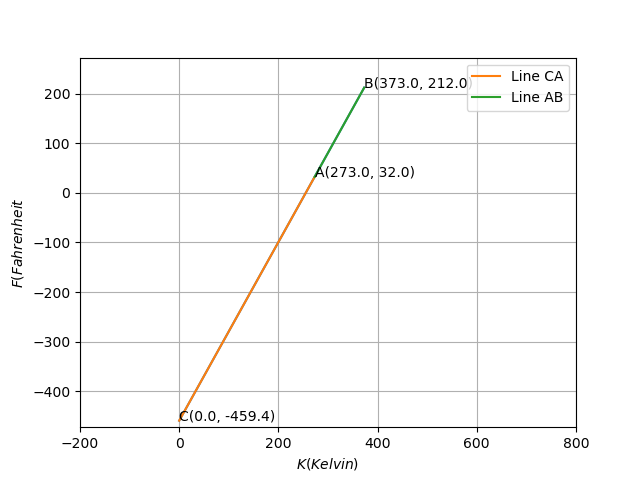
\includegraphics[width=\columnwidth, height=0.8\textheight, keepaspectratio]{../figs/fig.png}     
\end{frame}

\begin{frame}[fragile]
    \frametitle{C Code (0) - Importing libraries}

    \begin{lstlisting}
#include <stdio.h>
#include <stdlib.h>
#include <string.h>
#include <math.h>
#include <sys/socket.h>
#include <netinet/in.h>
#include <unistd.h>
#include "libs/matfun.h"
#include "libs/geofun.h"
    \end{lstlisting}
\end{frame}
\begin{frame}[fragile]
    \frametitle{C Code (1) - Function to Generate Points on a Line}

    \begin{lstlisting}

void point_gen(FILE *p_file, double **A, double **B, int rows, int cols, int npts){
    for(int i = 0; i <= npts; i++){
     double **output = Matadd(A, Matscale(Matsub(B, A, rows, cols), rows, cols, (double)i/npts), rows, cols);
     fprintf(p_file, "%lf, %lf\n", output[0][0], output[1][0]);
     freeMat(output, rows);
    }
}

    \end{lstlisting}
\end{frame}


\begin{frame}[fragile]
    \frametitle{C Code (2) - Function to write points b/w given points to a file}

    \begin{lstlisting}
void write_points(double x1, double y1, double x2, double y2, double x3, double y3, int npts){
    int m = 2;
    int n = 1;

    double **A = createMat(m, n);
    double **B = createMat(m, n);
    double **C = createMat(m, n);

    B[0][0] = x2;
    B[1][0] = y2;
    \end{lstlisting}
\end{frame}
\begin{frame}[fragile]
    \frametitle{C Code (2) - Function to write points b/w given 2 points to a file}

    \begin{lstlisting}
    A[0][0] = x1;
    A[1][0] = y1;
    
    C[0][0] = x3;
    C[1][0] = y3;
    
    FILE *p_file;
    p_file = fopen("plot.dat", "w");
    
    if(p_file == NULL)
        printf("Error opening one of the data files\n");
    \end{lstlisting}
\end{frame}

\begin{frame}[fragile]
    \frametitle{C Code (2) - Function to write points b/w given 2 points to a file}
    \begin{lstlisting}
    point_gen(p_file, C, B, m, n, npts);
    point_gen(p_file, C, A, m, n, npts);
    point_gen(p_file, A, B, m, n, npts);
    
    freeMat(A, m);
    freeMat(B, m);
    freeMat(C, m);
    
    fclose(p_file);
}
}
    \end{lstlisting}
\end{frame}

\begin{frame}[fragile]
    \frametitle{Python Code (0) - Importing libraries and checking system}
    \begin{lstlisting}
import numpy as np
import matplotlib.pyplot as plt
import ctypes
import os
import sys
import subprocess
import math

print('Using termux? (y/n)')
termux = input()
\end{lstlisting}
\end{frame}

\begin{frame}[fragile]
    \frametitle{Python Code (1) - Using Shared Object}
    \begin{lstlisting}
lib_path = os.path.join(os.path.dirname(__file__), 'plot.so')
my_lib = ctypes.CDLL(lib_path)

my_lib.write_points.argtypes = [ctypes.c_double, ctypes.c_double, ctypes.c_double, ctypes.c_double, ctypes.c_double, ctypes.c_double, ctypes.c_int]
my_lib.write_points.restype = None
A = np.array([273, 32]).reshape(-1, 1)
B = np.array([373, 212]).reshape(-1, 1)
C = np.array([0, -459.4]).reshape(-1, 1)
npts = 20000
\end{lstlisting}
\end{frame}

\begin{frame}[fragile]
    \frametitle{Python Code (2) - Loading points and plotting them}
    \begin{lstlisting}
my_lib.write_points(A[0][0], A[1][0], B[0][0], B[1][0], C[0][0], C[1][0], npts)

fig = plt.figure()
ax = fig.add_subplot(111)
labels = ['CB', 'CA', 'AB']
pts = np.block([A, B, C])
vertices = ['A', 'B', 'C']
for i,label in enumerate(labels):
    points = np.loadtxt('plot.dat', delimiter = ',', usecols=(0,1))[i*(npts+1):(i+1)*(npts+1)]
    if(i > 0):
        ax.plot(points[:, 0], points[:, 1], label = (f'Line {label}'))
    else:
        ax.plot(points[:, 0], points[:, 1])
    ax.text(pts[:, i][0], pts[:, i][1], s=f'{vertices[i]}({round(pts[:, i][0],3)}, {round(pts[:, i][1],3)})')
\end{lstlisting}
\end{frame}

\begin{frame}[fragile]
    \frametitle{Python Code (3) - Labelling plot}
    \begin{lstlisting}
        ax.set_xlabel('$K(Kelvin)$')
        ax.set_ylabel('$F(Fahrenheit)$')
        ax.legend(loc='best')
        ax.grid() 
        ax.axis('equal')
        ax.set_xlim([-200, 800])
        ax.set_ylim([-500, 300])
    \end{lstlisting}
\end{frame}

\begin{frame}[fragile]
    \frametitle{Python Code (4) - Saving and displaying plot}
    \begin{lstlisting}
fig.savefig('../figs/fig2.png')
print('Saved figure to ../figs/fig2.png')

if(termux == 'y'):
    subprocess.run(shlex.split('termux-open ../figs/fig2.png'))
else:
    subprocess.run(["open",  "../figs/fig2.png"])
\end{lstlisting}
\end{frame}

\begin{frame}{Plot-Using Both C and Python}
    \centering
    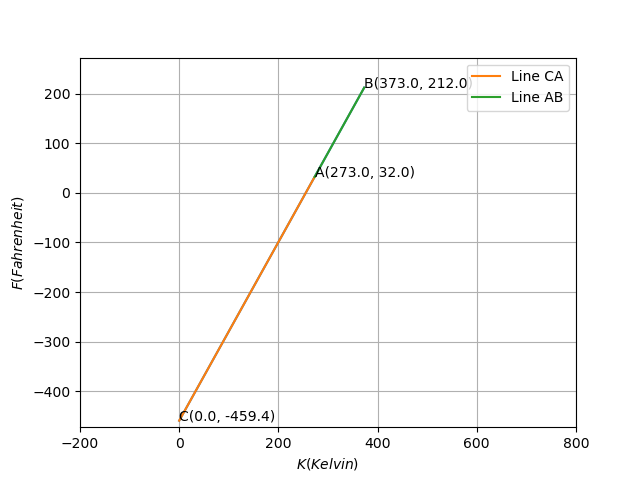
\includegraphics[width=\columnwidth, height=0.8\textheight, keepaspectratio]{../figs/fig2.png}     
\end{frame}

\end{document}